\section{Introduction}
Une fois la conception validée, il est temps de passer à la réalisation. Nous présentons dans ce chapitre le module réalisé en utilisant des captures d’écran pour montrer ses principales fonctionnalités. Nous commençons par présenter les outils et technologies utilisées pour le développement, ensuite nous passons à l’architecture technique de la solution puis l’architecture du code.

\section{Outils et Technologies utilisées pour le développement}

 \subsection{Spring}
 
  \subsubsection{Spring Framework }
  
  
  Spring Framework fournit un modèle complet de programmation et de configuration pour les applications d'entreprise modernes basées sur Java - sur tout type de plate-forme de déploiement.
  
  Un élément clé de Spring est le support infrastructurel au niveau de l’application: Spring met l’accent sur la «plomberie» des applications d’entreprise afin que les équipes puissent se concentrer sur la logique métier au niveau de l’application, sans liens inutiles avec des environnements de déploiement spécifiques.
  
 \subsubsection{Spring boot}
 Spring Boot makes it easy to create stand-alone, production-grade Spring based Applications that you can "just run".
 
 We take an opinionated view of the Spring platform and third-party libraries so you can get started with minimum fuss. Most Spring Boot applications need very little Spring configuration.
   \subsubsection{Spring Data}
   
 \subsubsection{Spring Cloud}
 Spring Cloud fournit aux développeurs des outils permettant de créer rapidement certains modèles courants dans les systèmes distribués (gestion de la configuration, découverte de services, disjoncteurs, routage intelligent, micro-proxy, bus de contrôle, jetons à usage unique, verrous globaux, élection des dirigeants, distribution sessions, état du cluster). La coordination des systèmes distribués conduit à des modèles de plaque de chaudière et, grâce à Spring Cloud, les développeurs peuvent rapidement mettre en service des services et des applications mettant en œuvre ces modèles. Ils fonctionneront bien dans n’importe quel environnement distribué, y compris l’ordinateur portable du développeur, les centres de données à nu et les plateformes gérées telles que Cloud Foundry.
 
 
  \subsubsection{Spring Cloud Netflix}
 Spring Cloud Netflix fournit des intégrations Netflix OSS pour les applications Spring Boot via la configuration automatique et la liaison à Spring Environment et à d'autres idiomes de modèles de programmation Spring. Quelques annotations simples vous permettent d'activer et de configurer rapidement les modèles courants dans votre application et de créer de grands systèmes distribués avec des composants Netflix testés au combat. Les modèles fournis incluent la découverte de service (Eureka), le disjoncteur (Hystrix), le routage intelligent (Zuul) et l’équilibrage de la charge côté client (ruban).
 
 \subsection{ Qu'est-ce que Micro Service?}

 L'objectif principal de la mise en œuvre des micro-services est de scinder l'application en un service distinct pour chaque fonctionnalité de base et chaque service de l'API. Elle devrait être déployée indépendamment sur le cloud. Nous avons choisi le langage de programmation réactif du projet familial spring.io avec un ensemble de composants pouvant être utilisés pour mettre en œuvre notre modèle d'exploitation. Spring Cloud intègre très bien les composants Netflix dans l’environnement Spring. Il utilise une configuration automatique et une convention de configuration similaire à celle du fonctionnement de Spring Boot.


\subsubsection{Pourquoi l’architecture de Microservices?}

Nous avons choisi l'architecture de micro-services pour écrire chaque fonctionnalité en tant que service distinct pour les fonctionnalités de base et d'API, ce qui nous aide à réaliser la livraison et l'intégration en continu.

\subsubsection{Patterns dans l'architecture des microservices}



\begin{itemize}
\item  \textbf{Api Gatway }


\begin{enumerate}
	
\item 	  Choisissez de créer l’application en tant qu’ensemble de micro-services.

\item	  Décidez comment le client de l'application va interagir avec les micro-services.

\item	  Avec une application monolithique, il n'y a qu'un seul ensemble de points d'extrémité (généralement répliqués, à charge équilibrée).

\item	  Dans une architecture de micro-services, chaque micro-service expose cependant un ensemble de
points finaux.
\end{enumerate}


\item \textbf{Service registry}

\begin{enumerate}
\item 	  Le registre de service aide à déterminer l’emplacement des instances de service pour envoyer la demande au correspondant
	un service
	
\item 	  Ici, nous avons utilisé Netflix Eureka pour enregistrer un service pouvant être enregistré dans le registre de services.
	serveur et il peut être identifié par le routeur.

	
\end{enumerate}
\item \textbf{Service Discovry}
\begin{enumerate}


\item   Dans une application monolithique, les services s'appellent par le biais d'appels de méthode ou de procédure au niveau de la langue.

\item   Toutefois, dans une application moderne basée sur des micro-services, elle s'exécute généralement dans des environnements virtualisés où le nombre
des instances d'un service et de leurs emplacements change de façon dynamique.

\item   Chaque service peut être identifié à l'aide d'un routeur enregistré auprès du serveur de registre de services.
	
\end{enumerate}
\end{itemize}



\subsubsection{Architecture des microservices via les composants Netflix}
Nous avons utilisé les composants Netflix pour réaliser les modèles d’architecture de microservices ci-dessus.\cite{MicroServices}.

% Please add the following required packages to your document preamble:
% \usepackage[table,xcdraw]{xcolor}
% If you use beamer only pass "xcolor=table" option, i.e. \documentclass[xcolor=table]{beamer}
% \usepackage[normalem]{ulem}
% \useunder{\uline}{\ul}{}
\begin{table}[H]
	\begin{tabular}{|l|l|}
		\hline
		\rowcolor[HTML]{5174DA} 
		{\color[HTML]{FFFFFF} \textbf{Operations Component}} & {\color[HTML]{FFFFFF} \textbf{Spring, Netflix OSS}} \\ \hline
		Service Discovery server & Netflix Eureka \\ \hline
		Edge Server & Netflix Zuul \\ \hline
		Central configuration server & Spring Cloud Config Server \\ \hline
		Dynamic Routing and Load Balancer & Netflix Ribbon \\ \hline
		OAuth 2.0 protected API’s & Spring Cloud + Spring Security OAuth2 \\ \hline
		Monitoring & Netflix Hystrix dashboard and turbine \\ \hline
	\end{tabular}
\end{table}

\subsection{Composantes majeures de Netflix}



\subsubsection{Service Discovery Server} 

\authorimg{images/ms-img04} Netflix Eureka permet aux micro-services de s’enregistrer eux-mêmes au moment de leur exécution, tels qu’ils apparaissent dans la structure du système.
\cite{MicroServices}


\subsubsection{Routage dynamique et équilibreur de charge} 

\authorimg{images/ms-img05}  Netflix Ribbon peut être utilisé par les consommateurs de services pour rechercher des services au moment de l’exécution. Le ruban utilise les informations disponibles dans Eureka pour localiser les instances de service appropriées. Si plusieurs instances sont trouvées, le Ruban appliquera un équilibrage de charge pour répartir les demandes sur les instances disponibles. Le ruban ne s'exécute pas en tant que service distinct, mais en tant que composant intégré dans chaque consommateur de service.\cite{MicroServices}





\subsubsection{Serveur Edge} 

\authorimg{images/ms-img06}  Zuul est (bien sûr) notre gardien du monde extérieur, ne permettant pas le passage de demandes externes non autorisées. Zulu fournit également un point d'entrée bien connu aux micro-services dans le paysage système. L'utilisation de ports alloués de manière dynamique est pratique pour éviter les conflits de ports et minimiser l'administration, mais elle rend évidemment la tâche plus difficile pour tout consommateur de services donné. Zuul utilise Ribbon pour rechercher les services disponibles et achemine la demande externe vers une instance de service appropriée.\cite{MicroServices}


\subsection{Spring Boot et Spring Cloud Netflix OSS – Micro Service Architecture}

\subsubsection{Micro Services avec Spring Boot}

 

Spring Boot est un tout nouveau framework de l'équipe de Pivotal, conçu pour simplifier le démarrage et le développement d'une nouvelle application Spring. Le cadre adopte une approche de configuration avisée, libérant les développeurs de la nécessité de définir la configuration standard.\cite{MicroServices}

\subsubsection{Spring Cloud Netflix}
 

Spring cloud Netflix fournit des intégrations Netflix OSS pour les applications de démarrage printanier via la configuration automatique et la liaison à l'environnement Spring et à d'autres modèles de programmation Spring. Avec quelques annotations simples, nous pouvons rapidement activer et configurer des modèles courants dans une application et construire des systèmes distribués volumineux avec des composants Netflix. De nombreuses fonctionnalités sont disponibles avec le nuage de printemps Netflix. Ici, nous avons répertorié certaines des fonctionnalités communes que nous avons implémentées avec les micro-services avec Spring Boot et Netflix,\cite{MicroServices}

\begin{itemize}
\item \textbf{Découverte du service:}
	
	Les instances Eureka peuvent être enregistrées et les clients peuvent
	Découvrez les exemples à l'aide de haricots à gestion printanière
	

\item \textbf{	Création de service:}	
	Le serveur Eureka intégré peut être créé avec
	configuration Java déclarative
	
\item \textbf{	Configuration Externel:}	
	
	Bridge from the Spring Environment (permet aux utilisateurs de
	configuration des composants Netflix à l'aide de Spring Boot
	conventions)
	
      \item \textbf{	Routeur et filtre:}	
	
	Enregistrement automatique des filtres Zuul, et un simple
	convention sur l'approche de configuration pour la création de proxy inverse.
\end{itemize}


\subsection{Maven} 
\subsubsection{Qu'est-ce que Maven ?}


Maven est essentiellement un outil de gestion et de compréhension de projet. 

Maven offre des fonctionnalités de :
\begin{itemize}
\item construction , compilation ;
\item documentation ;
\item  rapport ;
\item  gestion des dépendances ;
\item  gestion des sources ;
\item mise à jour de projet ;
\item  déploiement.
\end{itemize}

\subsubsection{Qu'est-ce que le POM ?}
Le \textbf{POM} (\textbf{P}roject \textbf{O}bject \textbf{M}odel) est une façon de décrire, de manière déclarative, un projet au sens de Maven. Cette description est contenue dans le fichier \textbf{pom.xml} présent dans le repertoire de base du projet. Le fichier pom.xml contient donc tous les éléments permettant de gérer le cycle de vie du projet. \cite{maven}.

Code xml :	
 \lstset{language=XML}
\begin{lstlisting}

<project xmlns="http://maven.apache.org/POM/4.0.0" xmlns:xsi="http://
www.w3.org/2001/XMLSchema-instance" xsi:schemaLocation="http://maven.
apache.org/POM/4.0.0 http://maven.apache.org/maven-v4_0_0.xsd"> 

<modelVersion>4.0.0</modelVersion> 
<groupId>com.mycompany.app</groupId> 
<artifactId>my-app</artifactId> 
<packaging>jar</packaging> 
<version>1.0-SNAPSHOT</version> 
<name>Maven Quick Start Archetype</name> 
<url>http://maven.apache.org</url> 

<dependencies> 
<dependency> 
<groupId>junit</groupId> 
<artifactId>junit</artifactId> 
<version>3.8.1</version> 
<scope>test</scope> 
</dependency> 
</dependencies> 

</project>

\end{lstlisting}

\begin{itemize}

\item \textbf{project} : c'est la balise racine de tous les fichiers pom.xml.
\item \textbf{modelVersion} : cette balise indique la version de POM utilisée. Bien que cette version ne change pas fréquemment, elle est obligatoire afin de garantir la stabilité d'utilisation.
\item \textbf{groupId} : cette balise permet d'identifier un groupe qui a créé le projet. Cette clé permet d'organiser et de retrouver plus facilement et rapidement le projet.
\item \textbf{artifactId} : cette balise indique un nom unique utilisé pour nommer les artifacts à construire.
\item \textbf{packaging} : type de packaging du projet ( ex. : JAR, WAR, EAR, etc.).
version : version de l'artifact généré par le projet.
\item \textbf{name} : nom du projet.
\item \textbf{url} : adresse du site du projet.
description : description du projet.
\item \textbf{dependencies} : balise permettant de gérer les dépendances.
\end{itemize}

\subsubsection{Qu'est-ce qu'un archetype ?}
Un archetype est un template de projet. Le fait d'utiliser des archetypes pour initialiser un projet permet de gagner du temps et de respecter une certaine convention. \cite{maven}.

\subsubsection{Qu'est-ce qu'une dépendance ?}
 Une dépendance est une référence vers un artefact spécifique contenu dans un repository. Cet artefact est nécessaire pour une ou plusieurs phases du cycle de vie du projet. \cite{maven}.
 
 L'exemple le plus simple est une dépendance sur une bibliothèque jar qui permet d'en utiliser le contenu dans le projet.\parencite{maven}.
 
 \subsubsection{Qu'est-ce qu'un artefact ?}
 
 Dans Maven, un artefact est un élément spécifique issu de la construction du logiciel. 
 
 Dans Java, les artefacts les plus communs sont des JARs, mais ce peut être aussi un fichier WAR, un EAR, un ZIP, etc.\parencite{maven}.

  
 
     \subsubsection{Qu'est-ce que le groupId/artifactId ?}
   Le groupId est l'identifiant du groupe, à l'origine du projet. GroupId suit les mêmes règles de nommage que les packages  Java (exemple : fr.masociete.monprojet), et on choisit généralement comme groupId le nom du top package du projet. \parencite{maven}.
   
   L'artifactId est l'identifiant du projet au sein de ce groupe. 
   
   L'artifactId est utilisé par défaut pour construire le nom de l'artefact final (exemple : pour un artifactId=monprojet, le nom du fichier jar généré sera monprojet-version.jar).  \subsubsection{Qu'est-ce qu'un SNAPSHOT ?}
 
    Par convention, une version en cours de développement d'un projet voit son numéro de version suivi d'un -SNAPSHOT. 
    
    Ainsi un projet en version 2.0-SNAPSHOT signifie que cette version est une pré-version de la version 2.0, en cours de développement. 
    
    Ce concept de SNAPSHOT est particulièrement important pour Maven. En effet, dans la gestion des dépendances, Maven va chercher à mettre à jour les versions SNAPSHOT régulièrement pour prendre en compte les derniers développements. 
    
    Utiliser une version SNAPSHOT permet de bénéficier des dernières fonctionnalités d'un projet, mais en contrepartie, cette version peut être (et est) appelée à être modifiée de façon importante, sans aucun préavis. \parencite{maven}.
       \subsubsection{Qu'est-ce que le repository local, distant ?}
    Un repository local est un répertoire sur le poste du développeur permettant de stocker, suivant la même arborescence, tous les artefacts téléchargés depuis le(s) repository distant(s). \cite{maven}.
    
    Un projet ayant pour POM :
    
    Code xml : 
 
     
    \lstset{language=XML}
    \begin{lstlisting}
    <project> 
    <modelVersion>4.0.0</modelVersion> 
    <groupId>fr.masociete</groupId> 
    <artifactId>monprojet</artifactId> 
    <version>1.0</version> 
    </project>
    \end{lstlisting}
    
    
    \subsection{bpmn js}
    
 
    bpmn-js est une boîte à outils de rendu et un modélisateur Web BPMN 2.0. Il est écrit en JavaScript, intègre les diagrammes BPMN 2.0 dans les navigateurs modernes et ne requiert aucun serveur. Cela facilite son intégration dans n’importe quelle application Web.
    
    La bibliothèque est construite de manière à pouvoir être à la fois un visualiseur et un modélisateur Web. Utilisez le visualiseur pour intégrer BPMN 2.0 dans vos applications et l'enrichir avec vos données. Utilisez le modélisateur pour créer des diagrammes BPMN 2.0 dans votre application. 
    
    
    \subsection{ Camunda BPM}
    Camunda BPM est un système de gestion de flux de travaux gratuit écrit en Java qui définit et exécute les processus métier dans BPMN 2.0. Camunda BPM prend également en charge les normes CMMN 1.1 et DMN 1.1 normalisées par le groupe de gestion des objets (OMG).  
    
    
    \subsection{Thymeleaf}
    
    Thymeleaf est un moteur de template Java moderne côté serveur pour les environnements Web et autonomes.
    
    L'objectif principal de Thymeleaf est d'intégrer des modèles naturels élégants à votre flux de travail de développement: un code HTML pouvant être correctement affiché dans les navigateurs et fonctionnant également en tant que prototypes statiques, ce qui permet de renforcer la collaboration au sein des équipes de développement.
    
    Avec des modules pour Spring Framework, une multitude d’intégrations avec vos outils favoris et la possibilité d’intégrer vos propres fonctionnalités, Thymeleaf est idéal pour le développement Web JVM HTML5 moderne - bien qu’il puisse faire beaucoup plus.
    
    
    
    \section{Architecture Modèle/Vue/Contrôleur}
    
    
  L'architecture Modèle/Vue/Contrôleur (MVC) est une façon d'organiser une interface graphique d'un programme. Elle consiste à distinguer trois entités distinctes qui sont, le modèle, la vue et le contrôleur ayant chacun un rôle précis dans l'interface.
  
  L'organisation globale d'une interface graphique est souvent délicate. Bien que la façon MVC d'organiser une interface ne soit pas la solution miracle, elle fournit souvent une première approche qui peut ensuite être adaptée. Elle offre aussi un cadre pour structurer une application.  
    
    Dans l'architecture MVC, les rôles des trois entités sont les suivants. \parencite{mvc}
    
    \begin{itemize}
    \item 	\textbf{modèle :} données (accès et mise à jour)
    \item 	\textbf{vue :} interface utilisateur (entrées et sorties)
    \item 	\textbf{contrôleur :} gestion des événements et synchronisation
    \end{itemize}

\subsection{Rôle du modèle}
    Le modèle contient les données manipulées par le programme. Il assure la gestion de ces données et garantit leur intégrité. Dans le cas typique d'une base de données, c'est le modèle qui la contient.
    
    Le modèle offre des méthodes pour mettre à jour ces données (insertion suppression, changement de valeur). Il offre aussi des méthodes pour récupérer ses données. Dans le cas de données importantes, le modèle peut autoriser plusieurs vues partielles des données. Si par exemple le programme manipule une base de données pour les emplois du temps, le modèle peut avoir des méthodes pour avoir, tous les cours d'une salle, tous les cours d'une personnes ou tous les cours d'une groupe de Td.
 \subsection{Rôle de la vue}
 La vue fait l'interface avec l'utilisateur. Sa première tâche est d'afficher les données qu'elle a récupérées auprès du modèle. Sa seconde tâche est de recevoir tous les actions de l'utilisateur (clic de souris, sélection d'une entrées, boutons, …). Ses différents événements sont envoyés au contrôleur.
 
 La vue peut aussi donner plusieurs vues, partielles ou non, des mêmes données. Par exemple, l'application de conversion de bases a un entier comme unique donnée. Ce même entier est affiché de multiples façons (en texte dans différentes bases, bit par bit avec des boutons à cocher, avec des curseurs). La vue peut aussi offrir la possibilité à l'utilisateur de changer de vue.
 \subsection{Rôle du contrôleur} 
 Le contrôleur est chargé de la synchronisation du modèle et de la vue. Il reçoit tous les événements de l'utilisateur et enclenche les actions à effectuer. Si une action nécessite un changement des données, le contrôleur demande la modification des données au modèle et ensuite avertit la vue que les données ont changé pour que celle-ci se mette à jour. Certains événements de l'utilisateur ne concerne pas les données mais la vue. Dans ce cas, le contrôleur demande à la vue de se modifier.
 
 Dans le cas d'une base de données des emplois du temps. Une action de l'utilisateur peut être l'entrée (saisie) d'un nouveau cours. Le contrôleur ajoute ce cours au modèle et demande sa prise en compte par la vue. Une action de l'utilisateur peut aussi être de sélectionner une nouvelle personne pour visualiser tous ses cours. Ceci me modifie pas la base des cours mais nécessite simplement que la vue s'adapte et offre à l'utilisateur une vision des cours de cette personne.
 
 Le contrôleur est souvent scindé en plusieurs parties dont chacune reçoit les événements d'une partie des composants. En effet si un même objet reçoit les événements de tous les composants, il lui faut déterminer quelle est l'origine de chaque événement. Ce tri des événements peut s'avérer fastidieuse et peut conduire à un code pas très élégant (un énorme switch). C'est pour éviter ce problème que le contrôleur est réparti en plusieurs objets.  
 \subsection{Interactions}
    Les différentes interactions entre le modèle, la vue et le contrôleur sont résumées par le schéma de la figure \ref{fig:mvc} suivante.
    
    
    
    
    
    
    
    
\begin{figure}[H]
	\centering
	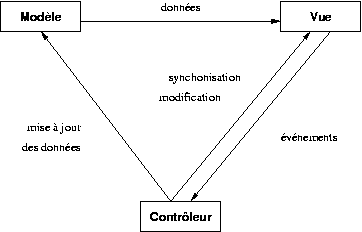
\includegraphics[width=0.6\linewidth]{images/mvc}
	\caption{Interactions entre le modèle, la vue et le contrôleur}
	\label{fig:mvc}
\end{figure}
    
    
    